% RISC Zero proving pipeline — grounded in: this thesis's prove logs
% (segment_preflight -> prove_segment_core -> verify_integrity, x131) and the
% RISC0 v3.0.x receipt API (lift / join / resolve / identity_p254; composite vs
% succinct). Compile standalone:  pdflatex risc0_pipeline.tex
\documentclass[border=4pt]{standalone}
\usepackage{tikz}
\usepackage{newtxtext,newtxmath}
\usetikzlibrary{positioning,arrows.meta,fit,backgrounds,calc}
\begin{document}
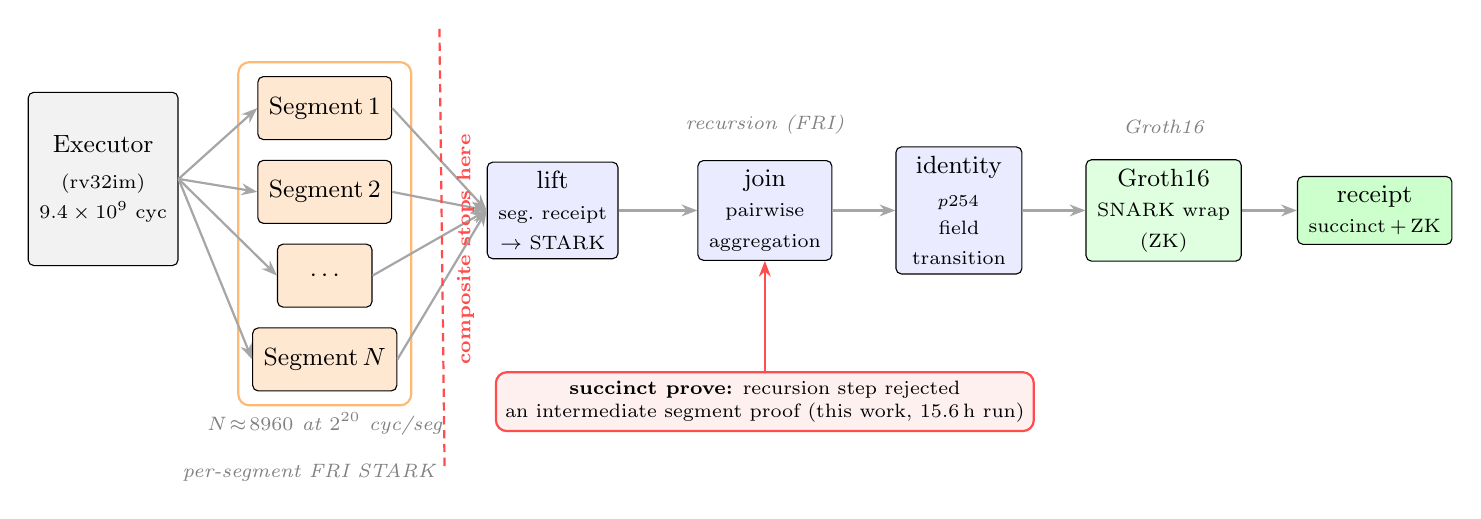
\begin{tikzpicture}[
  font=\small,
  >={Stealth[length=2mm]},
  box/.style={draw,rounded corners=2pt,minimum height=8mm,inner xsep=4pt,align=center},
  seg/.style={box,fill=orange!18,minimum width=12mm},
  rec/.style={box,fill=blue!8,minimum width=16mm},
  fin/.style={box,fill=green!12,minimum width=16mm},
  exec/.style={box,fill=gray!10,minimum width=16mm,minimum height=22mm},
  lbl/.style={font=\scriptsize\itshape,gray},
  flow/.style={->,thick,gray!70},
]

% --- Executor ---
\node[exec] (exec) {Executor\\[2pt]\scriptsize (rv32im)\\\scriptsize $9.4\times10^{9}$ cyc};

% --- per-segment STARK provers (FRI) ---
\node[seg,right=10mm of exec,yshift=9mm]  (s1) {Segment\,1};
\node[seg,below=2.5mm of s1]              (s2) {Segment\,2};
\node[seg,below=2.5mm of s2]              (s3) {$\cdots$};
\node[seg,below=2.5mm of s3]              (s4) {Segment\,$N$};
\node[lbl,below=1.5mm of s4] {$N\!\approx\!8960$ at $2^{20}$ cyc/seg};

% --- lift: segment receipt -> recursion receipt ---
\node[rec,right=12mm of s1,yshift=-13mm] (lift) {lift\\\scriptsize seg.\ receipt\\\scriptsize $\to$ STARK};

% --- join tree (pairwise recursion) ---
\node[rec,right=10mm of lift] (join) {join\\\scriptsize pairwise\\\scriptsize aggregation};

% --- resolve / identity ---
\node[rec,right=8mm of join] (idn) {identity\\$_{p254}$\\\scriptsize field\\\scriptsize transition};

% --- Groth16 wrap ---
\node[fin,right=8mm of idn] (g16) {Groth16\\\scriptsize SNARK wrap\\\scriptsize (ZK)};
\node[box,right=7mm of g16,fill=green!20,minimum width=11mm] (out) {receipt\\\scriptsize succinct\,+\,ZK};

% --- arrows ---
\foreach \s in {s1,s2,s3,s4} \draw[flow] (exec.east) -- (\s.west);
\foreach \s in {s1,s2,s3,s4} \draw[flow] (\s.east) -- (lift.west);
\draw[flow] (lift) -- (join);
\draw[flow] (join) -- (idn);
\draw[flow] (idn) -- (g16);
\draw[flow] (g16) -- (out);

% --- layer brackets (FRI / FRI / Groth16) ---
\begin{scope}[on background layer]
  \node[fit=(s1)(s4),draw=orange!55,thick,rounded corners,inner sep=5pt] (frbox) {};
\end{scope}
\node[lbl,below=8mm of s4,xshift=-2mm] {per-segment FRI STARK};
\node[lbl,above=2mm of join] {recursion (FRI)};
\node[lbl,above=2mm of g16] {Groth16};

% --- THESIS-SPECIFIC annotations: composite stops here; succinct continues; failure point ---
\draw[densely dashed,red!70,thick]
  ($(s1.north east)+(6mm,6mm)$) -- ($(s4.south east)+(6mm,-10mm)$);
\node[font=\scriptsize\bfseries,red!70,align=center,rotate=90]
  at ($(s1.north east)!0.5!(s4.south east)+(9mm,-2mm)$) {composite stops here};
\node[draw=red!70,thick,rounded corners,fill=red!6,font=\scriptsize,align=center,
      below=14mm of join] (fail)
  {\textbf{succinct prove:} recursion step rejected\\an intermediate segment proof
   (this work, $15.6$\,h run)};
\draw[red!70,->,thick] (fail) -- (join);

\end{tikzpicture}
\end{document}
